\chapter{Flash Analysis}
\label{chp:Flash_Analysis}
explain goals (use the device to capture flashes, extract features and send them to the analyser)


\section{Flash characteristics}
\label{sec:Flash_characteristics}

\begin{figure}
	\centering     %%% not \center
	\label{fig:Flashcapturing}
	\subfigure[Test setup in illuminated environment]{\label{fig:a}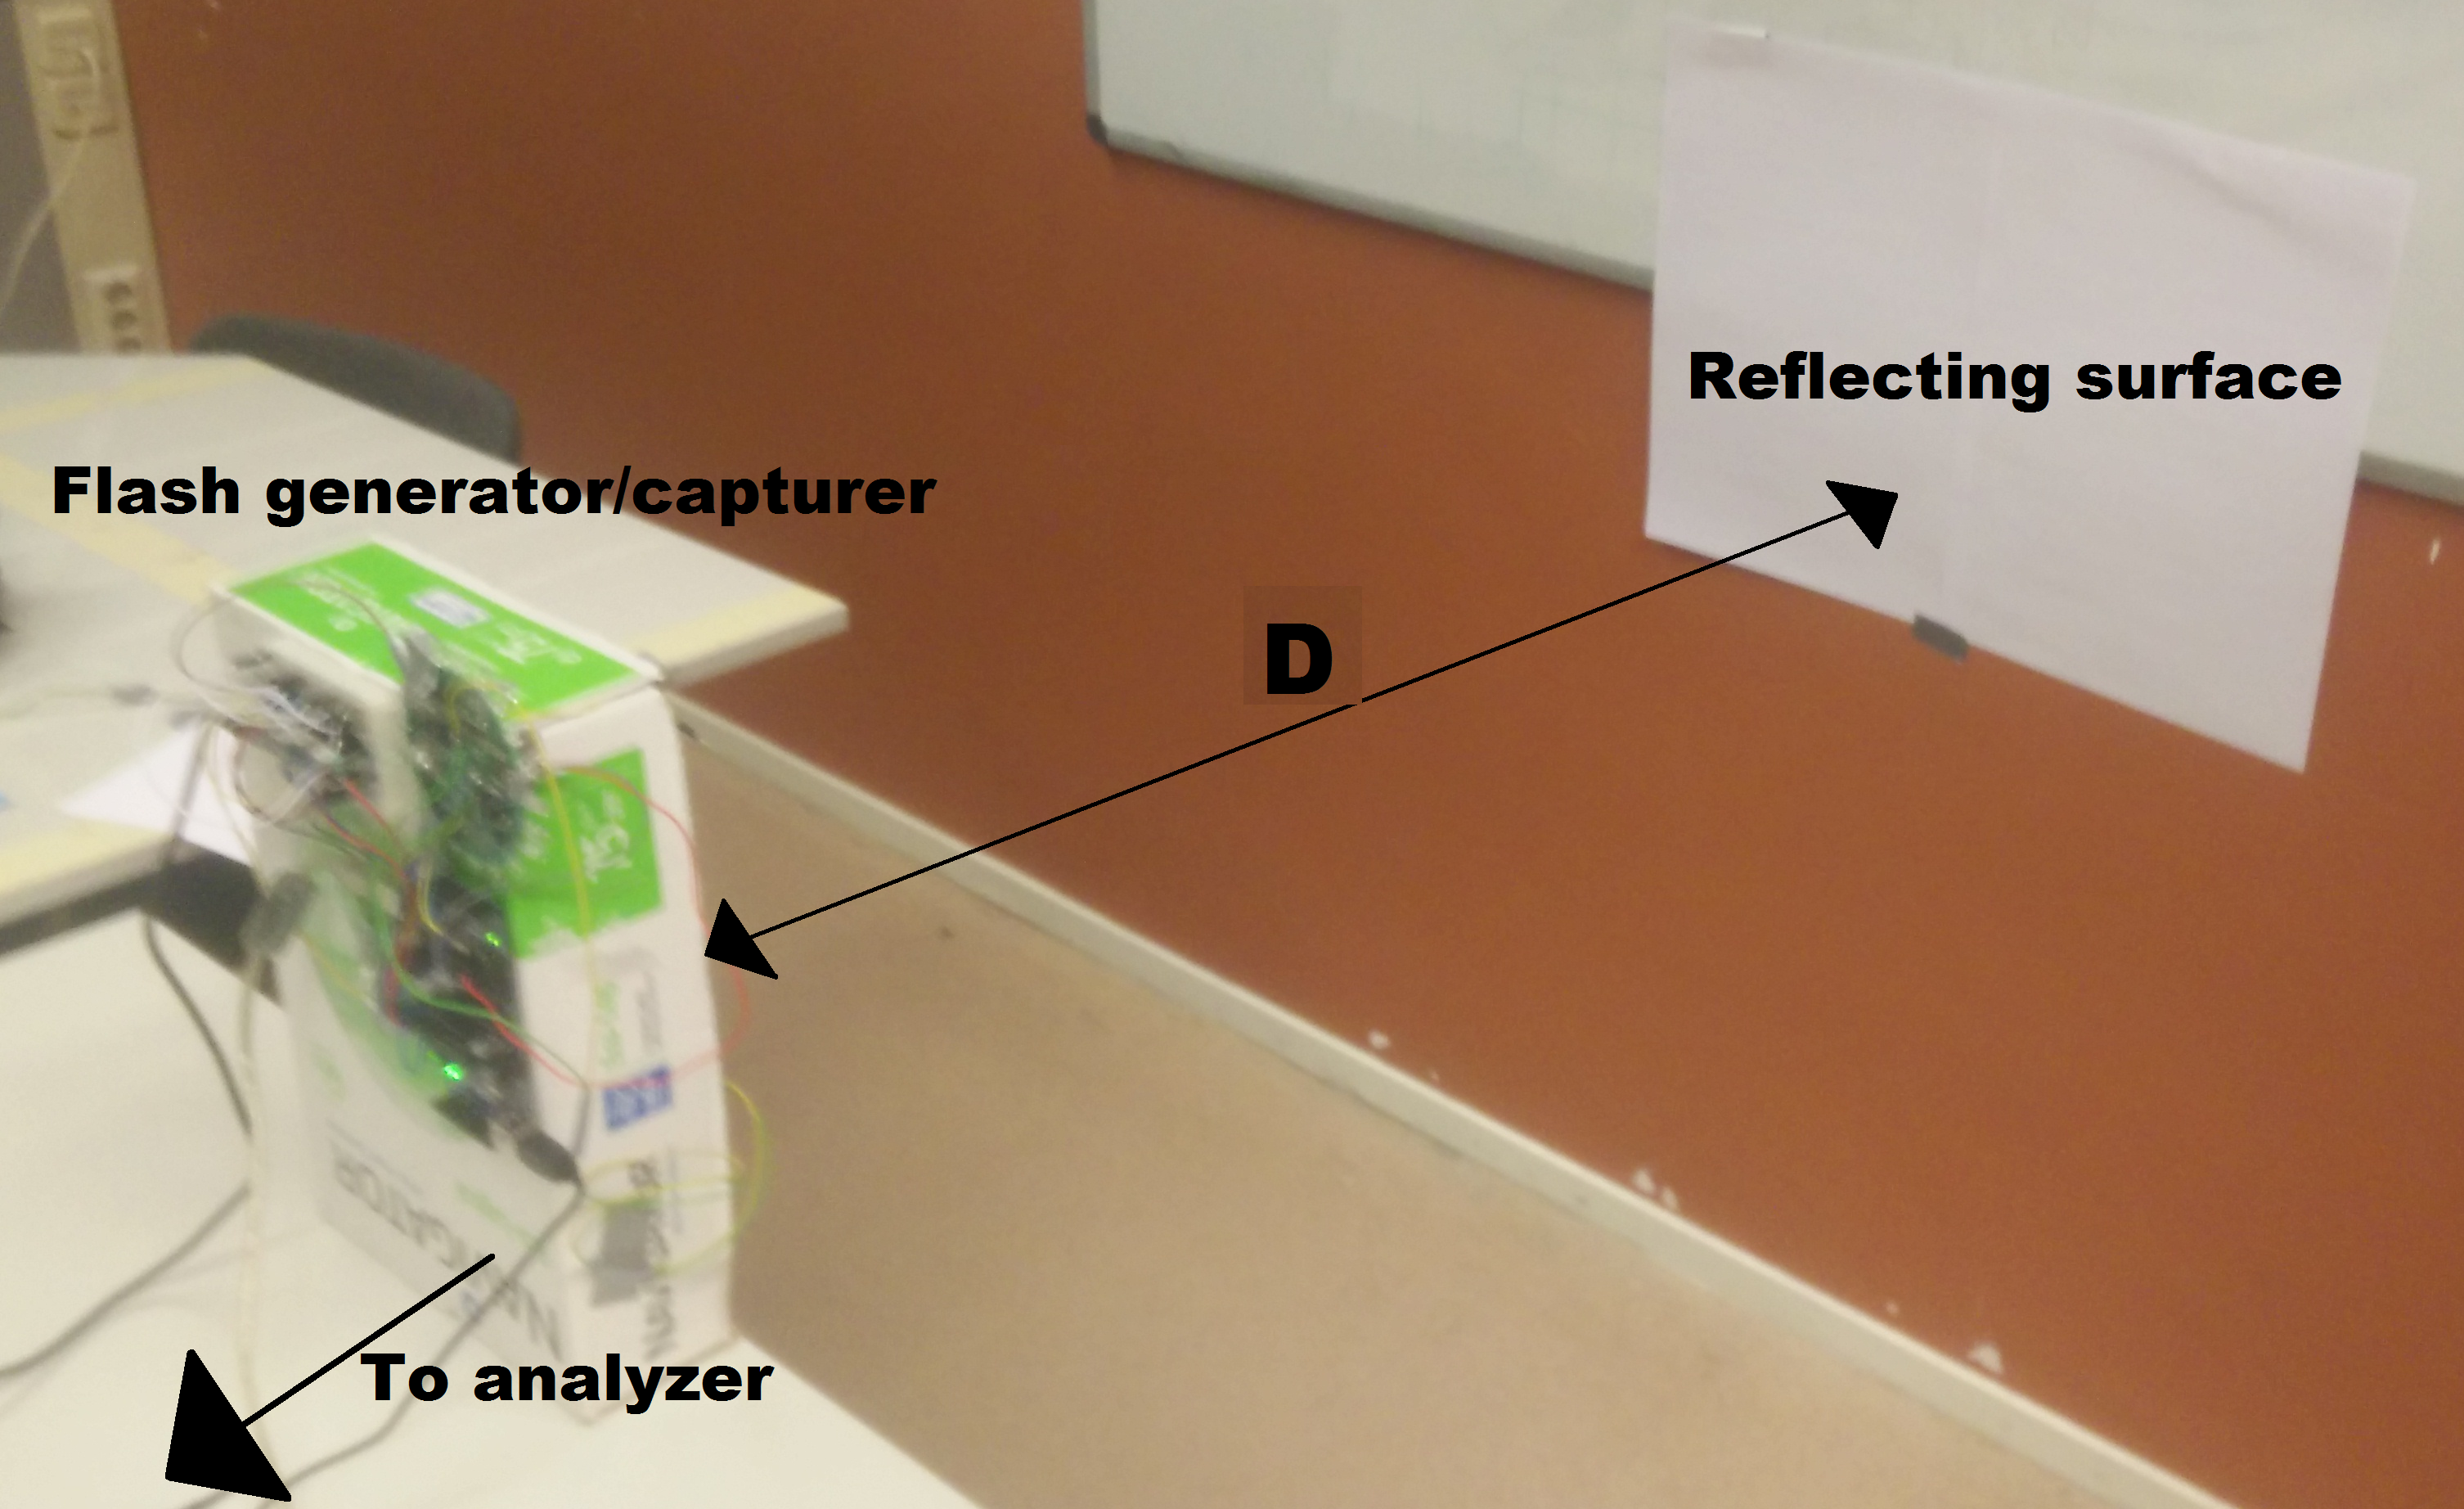
\includegraphics[width=60mm]{pics/Flashcapture_light.png}}
	\subfigure[Test setup in dark environment]{\label{fig:b}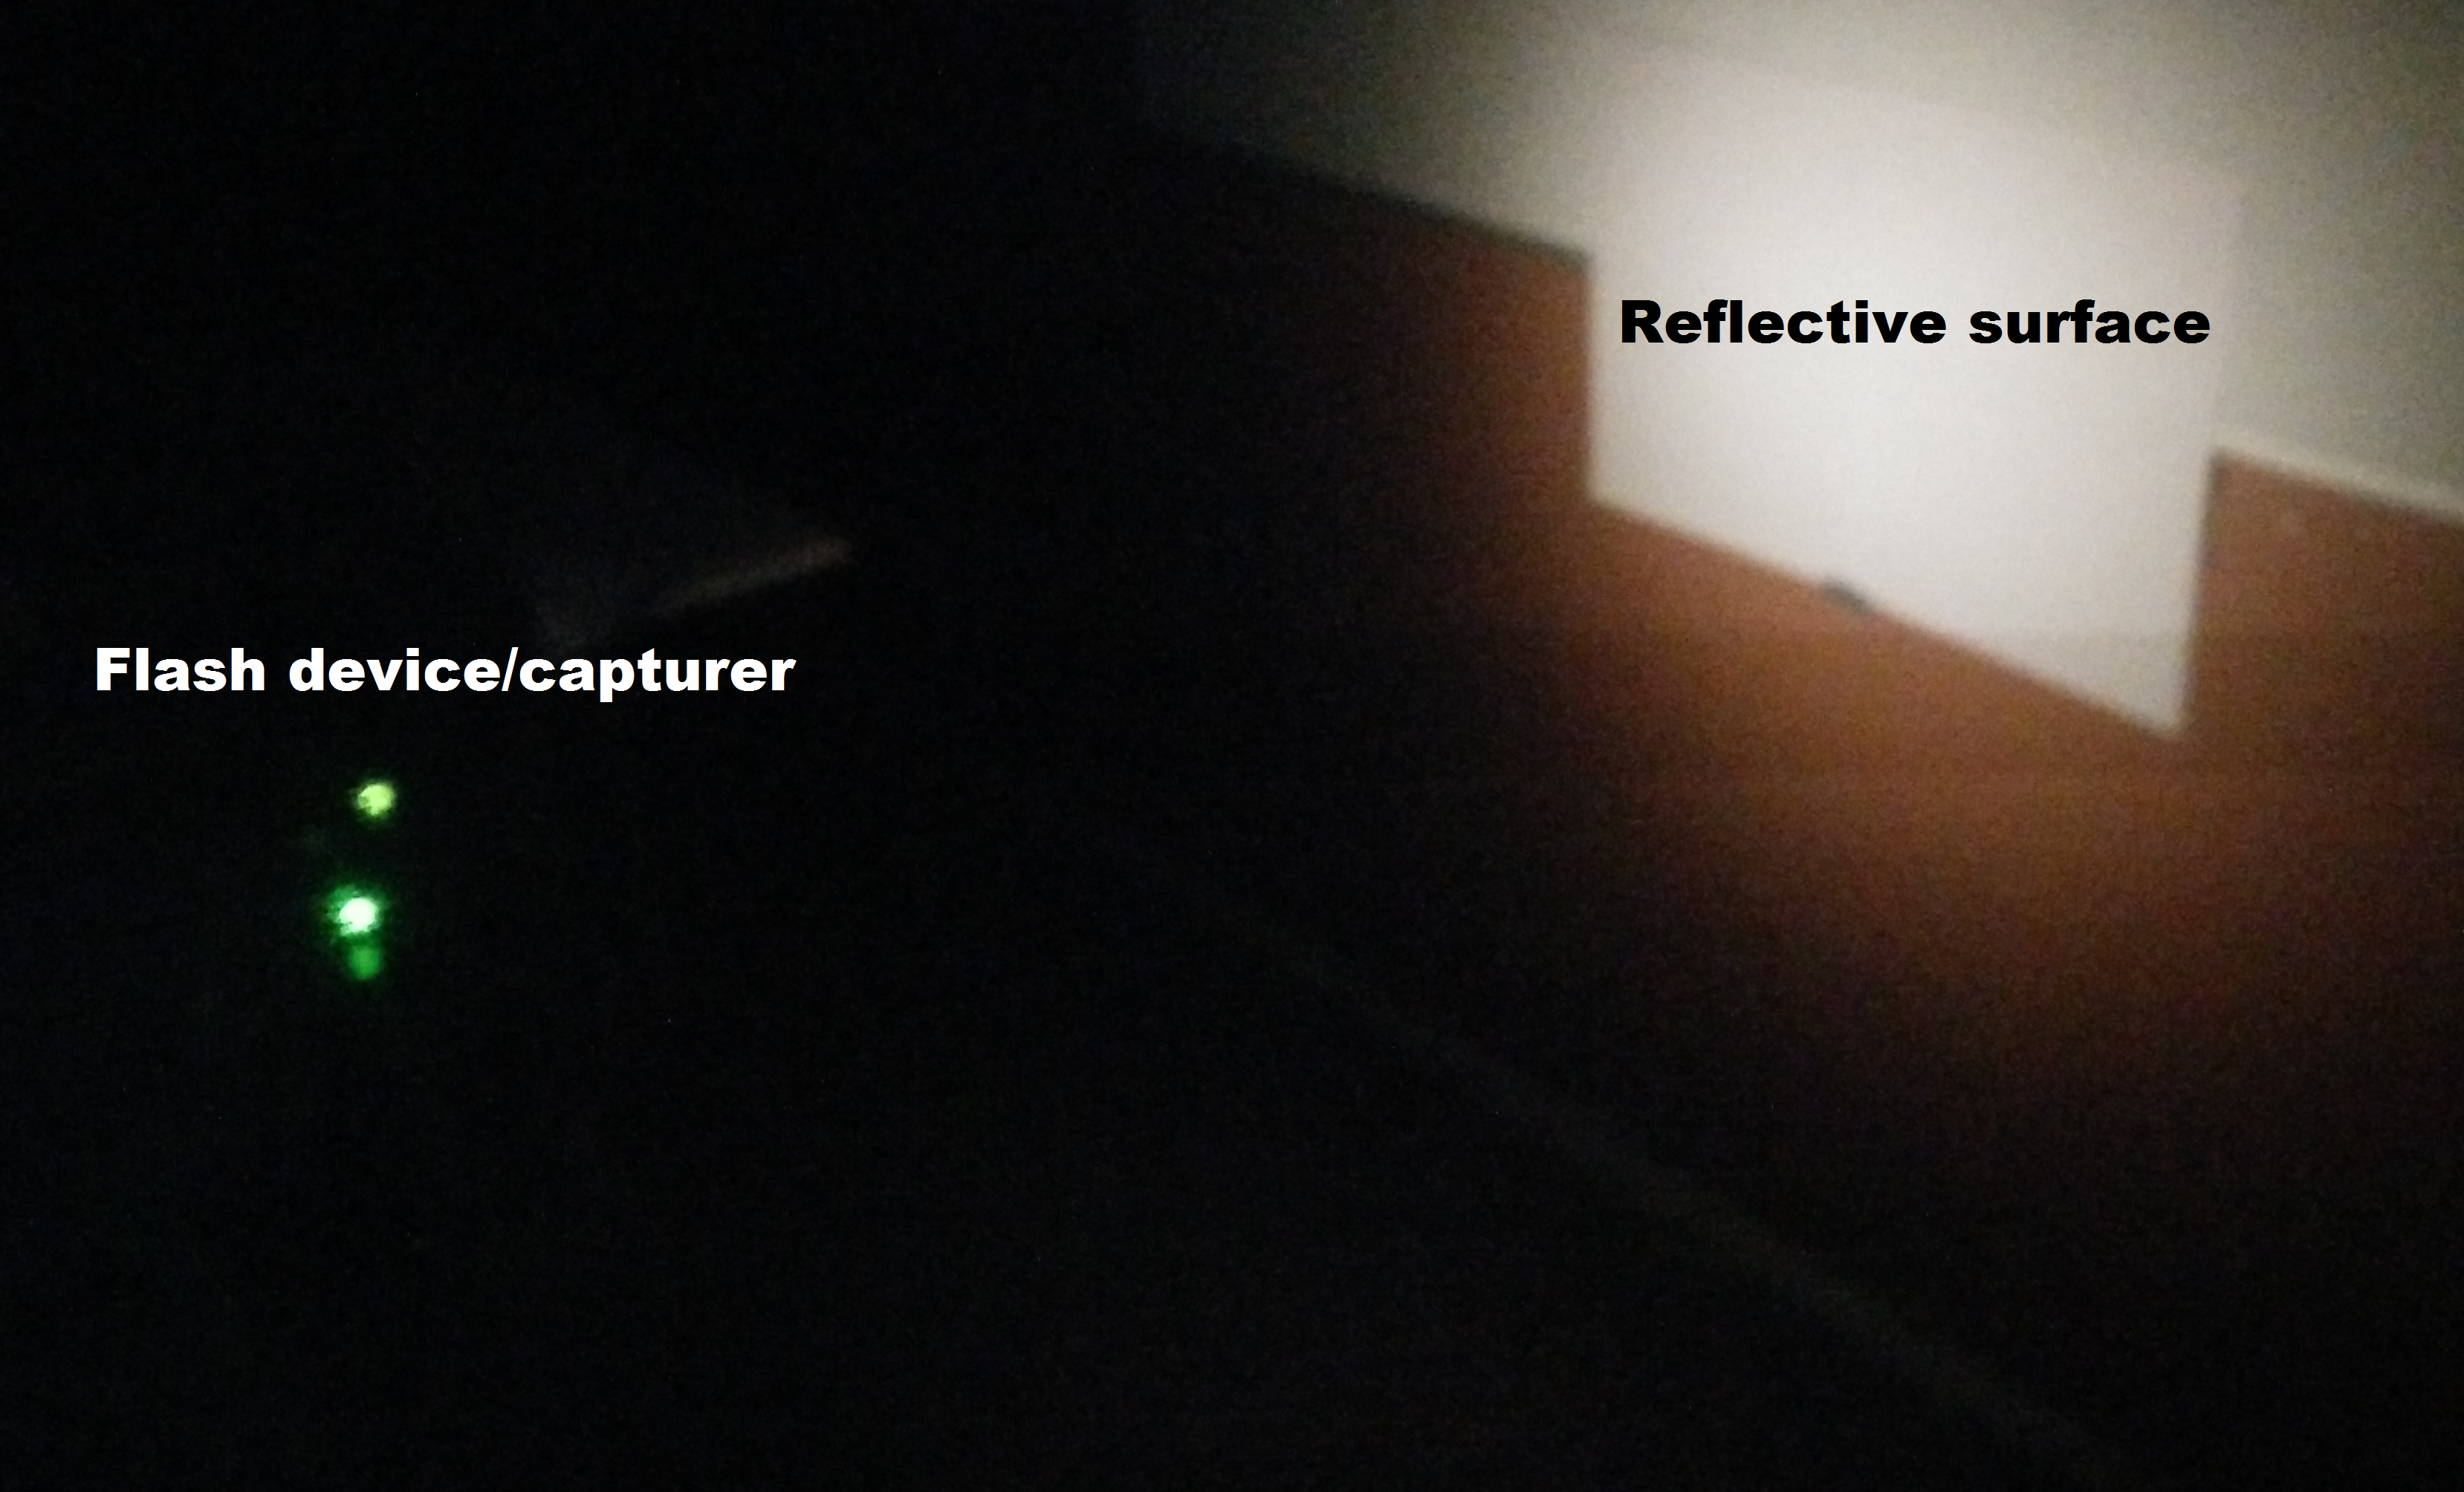
\includegraphics[width=60mm]{pics/Flashcapture_dark.png}}
	\caption{Test setup used to capture flashes in the darkroom.}
\end{figure}

show several captured flashes. and explain what we see.
explain features extractable from the flash
 - maximum
 - minimum
 - surface under graph
 - 

show real turn on delay time (or in our case, the time we are able to sense the light), rise-time, and turn-off-delay.
Define turn on time.

\begin{figure}[!h]
	\includegraphics[width=\textwidth]{pics/66KhzFilter_placeholder.png}
	\caption{The data captured by the system before and after filtering. @=PLACEHOLDER FIGURE!@.}
	\label{fig:66KhzFilter}
\end{figure}

\subsection{Data generation}
\label{sec:Data_generation}
Show several filtered captured signals in one figure\\
point out the part where light becomes constant\\
pick that t-on time as minimum\\
Mention that a sample of darkness can be taken @ 80 samples.\\
That the number (80) can be reduced by picking a FIR filter instead (less ripple)\\

\subsection{Results and conclusion}
\label{sec:conclusion}
Show the result of several "filtered flashes\\
Explain sources of the "noise", also show FFT and histogram of the noise\\
Explain that the noise could be reduced, but that this would cost a lot more processor time. (which is not recommended to run at 125Hz).\\
Note the noise is approximately Gaussian.

\begin{figure}[!h]
	\includegraphics[width=\textwidth]{pics/histogram_noise_placeholder.png}
	\caption{Histogram of the noise of the data sampled by the system. The distribution roughly follows a normal curve. @=PLACEHOLDER FIGURE!@.}
	\label{fig:histogram_noise}
\end{figure}
